 %\pdfoutput=1
\documentclass[conference]{IEEEtran}
\IEEEoverridecommandlockouts
% The preceding line is only needed to identify funding in the first footnote. If that is unneeded, please comment it out.
\usepackage[T1]{fontenc}
\usepackage{cite}
%\usepackage{caption}
%\usepackage{subcaption}
\usepackage{mathtools}
\usepackage{stackengine}
\def\delequal{\mathrel{\ensurestackMath{\stackon[1pt]{=}{\scriptstyle\Delta}}}}
\usepackage{amsmath,amssymb,amsfonts}
\usepackage{amsmath,epsfig,cite,amsfonts,amssymb,psfrag,subfigure}
\usepackage{graphicx}
\usepackage{blindtext}
\usepackage{textcomp}
\usepackage{xcolor}
\usepackage{algorithm}
\usepackage[noend]{algpseudocode}
\usepackage{amsthm}
\def\BibTeX{{\rm B\kern-.05em{\sc i\kern-.025em b}\kern-.08em
    T\kern-.1667em\lower.7ex\hbox{E}\kern-.125emX}}
\allowdisplaybreaks
\newtheorem{remark}{Remark}
\newtheorem{theorem}{Theorem}
\newtheorem{lemma}{Lemma}
\newtheorem{proposition}{Proposition}
\newtheorem{corollary}{Corollary}
\newcommand{\diag}{\mathop{\mathrm{diag}}}
\DeclareMathOperator{\E}{\mathbb{E}}
\usepackage[margin=0.7in]{geometry}
\usepackage[export]{adjustbox}
\setlength{\columnsep}{11mm}
\begin{document}

\title{Resource Allocation in an Open RAN System using Network Slicing\vspace{-.1cm}
}

\author{\IEEEauthorblockN{1\textsuperscript{st} Mojdeh Karbalaee Motalleb}
\IEEEauthorblockA{\textit{Electrical and Computer Engineering} \\
\textit{Tehran University}\\
Tehran, Iran \\
mojdeh.karbalaee@ut.ac.ir}
\and
\IEEEauthorblockN{2\textsuperscript{nd} Vahid Shah-Mansouri}
\IEEEauthorblockA{\textit{Electrical and Computer Engineering} \\
\textit{Tehran University}\\
Tehran, Iran \\
vmansouri@ut.ac.ir}
%\and
%\IEEEauthorblockN{3\textsuperscript{rd} Salar Nouri Naghadeh}
%\IEEEauthorblockA{\textit{Electrical and Computer Engineering} \\
%\textit{Tehran University}\\
%Tehran, Iran \\
%salar.nouri@ut.ac.ir}
%}
%  \author{
%    \IEEEauthorblockN{Mojdeh Karbalaee Motalleb, Vahid Shah-mansouri}
%    \IEEEauthorblockA{School of ECE, College of Engineering, University of Tehran, Iran \\
%    Email: \{mojdeh.karbalaee, vmansouri\}@ut.ac.ir,
%    \vspace{-.2cm}
%  }
 }

\maketitle

\begin{abstract}
Taking advantage of both virtual RAN (v-RAN) and Cloud RAN (C-RAN), Open RAN (O-RAN) is introduced as the next generation of RAN systems which leads to increase flexibility, Openness, and reduce operational costs and allow them to add new capabilities to the network more quickly.
O-RAN separate RAN into three different units, namely Radio Unit (O-RU), Distributed Unit (O-DU), and Central Unit (O-CU).
In this paper, we study the problem of baseband resource allocation and virtual network function (VNF) activation in O-RAN architecture based on their service priority for a different types of 5G services includes enhanced mobile broadband (eMBB), ultra-reliable low latency communications (URLLC) and massive Machine Type Communications (mMTC) services.
According to the concept of network slicing, the isolation of different types of services in O-DU, O-CU, and user plane function (UPF) is performed.
Limited fronthaul capacity and the restriction of end-to-end delay are considered in the problem.
The optimization of baseband resources includes O-RU assignment, physical resource block (PRB), and power allocation. The main problem is mixed-integer non-linear programming that is tremendously difficult.
To solve the challenging problem, we broke it down into two different steps that the iterative algorithm solves.
In the first step, we reformulated and simplified the problem to find the power allocation, PRB assignment, and the number of activated VNFs. In the second step, the O-RU association is carried out.
The proposed method is confirmed by the simulation results in a way that
the simulations illustrate a higher achievable data rate than a baseline scheme that only optimizes one of the baseband resources.
   
\end{abstract}

\begin{IEEEkeywords}
Open Radio Access Network (O-RAN), Virtual Network Function (VNF) 
\end{IEEEkeywords}

\section{Introduction} 
One of the goals of the fifth generation of wireless system is to achieve the desired QoS (such as rate, delay, power, ...) for different type of services. Network slicing is the best solution for this aim.
A network slice is an end-to-end logical network
which offers services with special needs. 
Multiple isolated network slices run, manage
,and work independently on the same infrastructure. There are several implementations of network slicing, including network core slicing, RAN slicing, and slicing of both sections. 
Different type of services includes enhanced mobile broadband (eMBB) and ultra-reliable low latency communications (URLLC) and massive Machine Type Communications (mMTC) services are introduced in 5th generation of mobile network. Each type of service requires special slice of network based on its QoS
 \cite{shen2020ai,setayesh2020joint,popovski20185g}.

Recently, RAN virtualization attracts significant attention from  both industry and academia since it 
has remarkable benefits which leads to increase the flexibility and 
reduce operator costs
such as CAPEX and OPEX and also allow them to add new capabilities to the network more quickly.
In addition to RAN virtualization, openness and RAN intelligence are two other fundamental points that encourage Open Radio Access Network (O-RAN)
Alliance to establish O-RAN as a next generation of RAN systems. 
The idea of O-RAN comes from the integration of virtual RAN (vRAN) and cloud RAN (CRAN) and it takes the advantage of both.
CRAN, divides RAN into two parts radio remote head (RRH) and base band unit (BBU). 
More than one distributed RRHs can be connected to a centralized BBU which is named BBU-pool\cite{han2019research}.
Unlike previous generation of RAN that divide RAN into two parts, O-RAN separate RAN into three different units, namely Radio Unit (O-RU), Distributed Unit (O-DU) and
Central Unit (O-CU).
O-RU is a logical node contains RF and lower PHY. Moreover, the O-DU expresses another logical node that includes higher PHY, MAC and RLC. In addition, the O-CU depicts the logical node contains two parts, which are O-CU user plane (O-CU-UP) and O-CU control plane (O-CU-CP). O-CU-UP hosts PDCP-UP and SDAP and
O-CU-CP hosts PDCP-CP and RRC.
O-DU and O-CU are connected to each other via an open and well-defined interface $F_1$.
Moreover, O-DU is connected to radio unit (O-RU) with an open fronthaul interface.
The architecture of O-RAN contains other principal logical nodes called Orchestration and Automation,
RAN Intelligent Controller (RIC)- Near Real Time and O-Cloud. 
One of the necessities of new generation of wireless networks is its intelligence.
Based on the requirement of smart wireless network, O-RAN offers machine learning techniques.
The two logical nodes RIC-Non Real Time (which is placed in Orchestration and Automation node) and RIC- Near Real Time implement the algorithms for network intelligence 
\cite{gavrilovska2020cloud,niknam2020intelligent,kazemifard2021minimum,both2021system,ORANArch,ORANML,lin2021toward}.

To improve system performance in the fifth generation of telecommunications, the separation of network software and hardware elements has been done and introduced as network function virtualization (NFV), and virtual network functions (VNF) are system function blocks. The key idea of the implementation of NFV is 
to decouple software from physical hardware, dynamic scaling and the deployment of flexible network function. A usual NFV offer is to execute VNFs on a virtual machines or containers in a cloud system \cite{mijumbi2015network, luo2020online}.
As a result, some O-RAN components that includes user plane function (UPF) , O-CU, O-DU and RAN Intelligent Controller (RIC)-near real time, are virtualized and implemented as a VNF that can be run on virtual machines (VMs) or containers.
\subsection{Related Works}
Network slicing is increasingly receiving research attention.
Many researcher, studied the problem of resource allocation in network slicing for multitenant cellular networks \cite{feng2020dynamic,lee2018dynamic,lee2016new}.
In \cite{lee2018dynamic},
dynamic network slicing in multitenant heterogeneous CRAN (H-CRAN) is considered. The process of allocating network resources to users is discussed. The network slicing scheme includes a higher level, which manages user acceptance control, user communication which includes radio unit association (RRH association to maximize user rates and allocate base band resource capacity), the allocation of BBU capacity and a lower level, which is the allocation of power and physical resource blocks (PRB) among users. 
In article \cite{xiang2020realization}, network slicing in the radio section is considered for fog or F-RAN structure, in which two network slices are set for hotspots and vehicle scenarios with related infrastructure. In \cite{elayoubi20195g,d2020toward} the implementation of RAN level slicing is discussed in mobile network operator (MNO). Also the problem of resource allocation is considered. 
Moreover, the challenges facing RAN slicing have also been explored, one of which involves designing and managing multiple slices in the shared infrastructure in an efficient manner while guaranteeing the agreed 
service level agreement (SLA) for each.

Multiplexing of eMBB and URLLC services on the same RAN and sharing the resources for these services is a challenging problem that many researchers pay attention to this topic. In \cite{setayesh2020joint,yang2020should}
the problem of resource allocation in the coexistence of these two services (URLLC and eMBB) is considered
based on their QoS. In \cite{alsenwi2021intelligent}, the problem of resource allocation for joint eMBB and URLLC is formulated and solved by deep reinforcement learning. In \cite{saggese2021power}
the problem of power minimization for these two type services (URLLC and eMBB) is presented for non-orthogonal multiple access (NOMA) and orthogonal multiple access (OMA). In \cite{korrai2020ran},
the authors proposed to allocate RAN resources for the network slicing system in the coexistence of eMBB and URLLC services. The system guarantee the latency, the service rate and the  maintenance of the reliability.

Virtualization technique for RAN and core is one of the interested topics.  
In \cite{SystemCostMinimization,guo2016exploiting}, the authors solve the problem of obtaining beamforming and VMs activation 
in C-RAN system with limited fronthaul capacity. The goal of this paper is to minimize the energy cost, with the system delay, fronthaul capacity and rate constraint. To guarantee delay for services, transmission and processing delay is modeled based on M/M/1 queuing theory. In \cite{luong2018joint,luong2018novel}, the problem of joint virtual computing resource allocation with beamforming is formulated; Also the association of RRH to UE is considered and solved using novel methods.
In \cite{ali2019energy,ali2019energy1,ali2018joint}, the problem of joint power allocation and RRH association in H-CRAN system is considered to maximize energy efficiency.
\subsection{Main Contribution}
The aim of this study is to jointly optimize VNF activation, power allocation, PRB allocation ,and O-RUs association to develop an isolated network slicing outline for different type of services in an O-RAN platform. In this paper, as  depicted in Figure \ref{fig:c11}, the downlink of the ORAN system is studied.
The main contributions of this paper are summarized as follow:
\begin{itemize}
\item In this paper a network slicing model is depicted for three different type of services introduced in 5G (URLLC, eMBB and mMTC) and the problem of radio resource allocation and VNF activation is studied in the O-RAN architecture.
We formulate the problem of baseband resource allocation to maximize the weighted throughput of O-RAN system for different type of services with specific QoS. 
\item The desired QoS conditions such as delay and throughput are considered for different type of services. We formulate the end-to end mean delay of system based on the activated VNFs and the throughput of each user.
We take into account the limited fronthaul capacity and accurately obtain the power and the capacity of each O-RU based on the quantization noise.
We model the interference of neighboring O-RU and formulate the accurate throughput
for different type of services. We model the throughput of URLLC and mMTC based on their short packet transmission.
\item The main problem is a mixed-integer non linear programming that is extremely difficult to solve.
We perform a two-step iterative algorithm to solve it.
The two-step iterative algorithm is presented for the resource management framework with the first-step VNF activation, power allocation and PRB association and the second-step O-RU association.
\item For the first-step, we reformulate and simplificate the main problem to find an upper and lower bound for number of activated VNFs and using lagrangian function and KKT conditions to find optimal power and PRB allocation.
For the second-step, the problem of O-RU association can be convert to a multiple knapsack problem and solved by Greedy algorithm.
\end{itemize}  

\begin{figure*}
  \centering 
    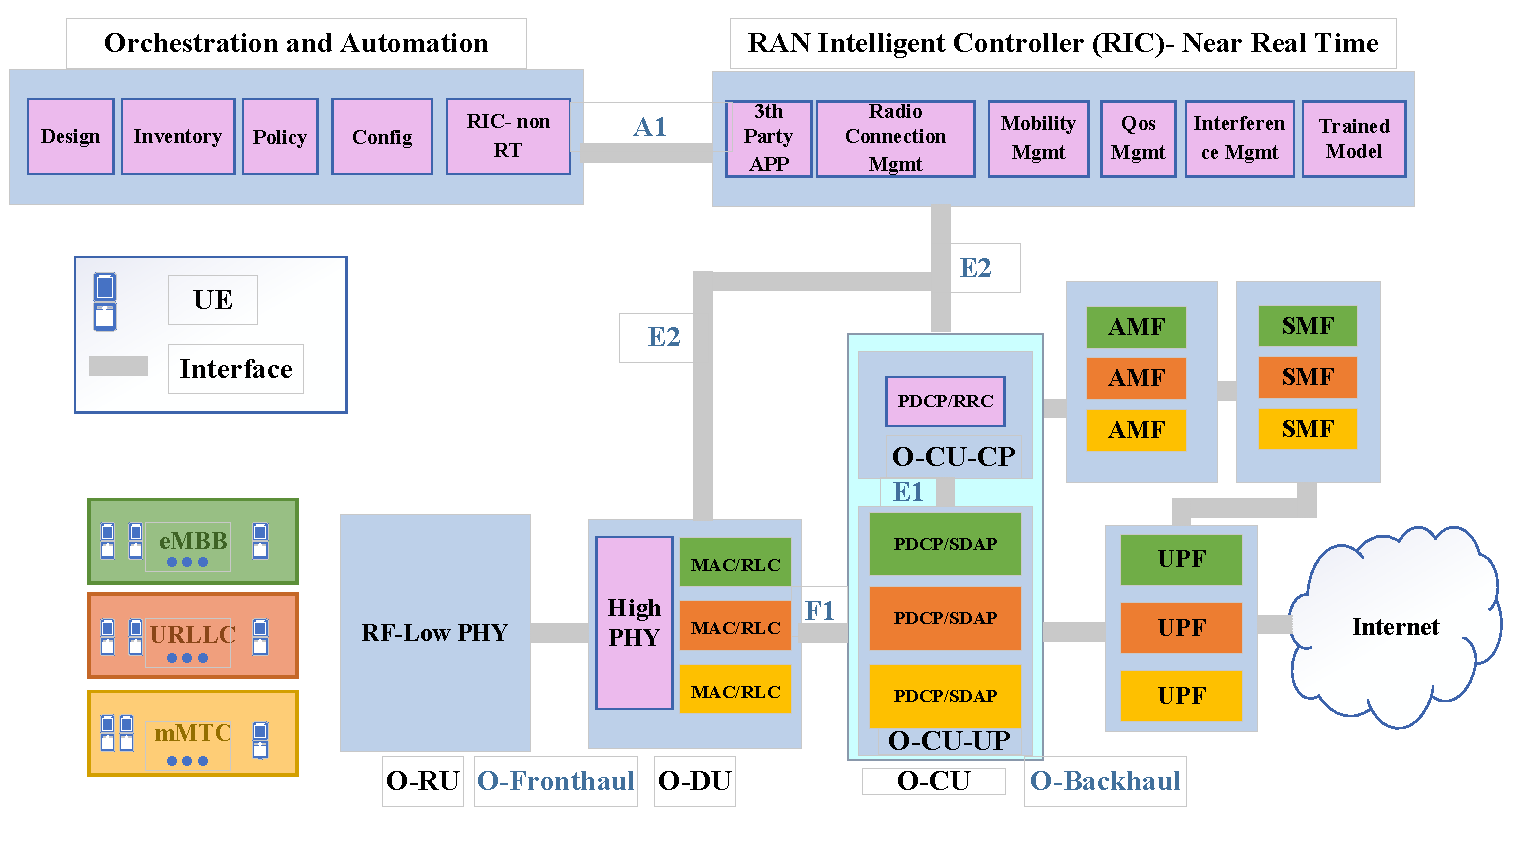
\includegraphics[scale = 0.75]{finalDraw.pdf}
    %\includegraphics[max height=30cm,max width=9.5cm]{Drawing15.eps}
    %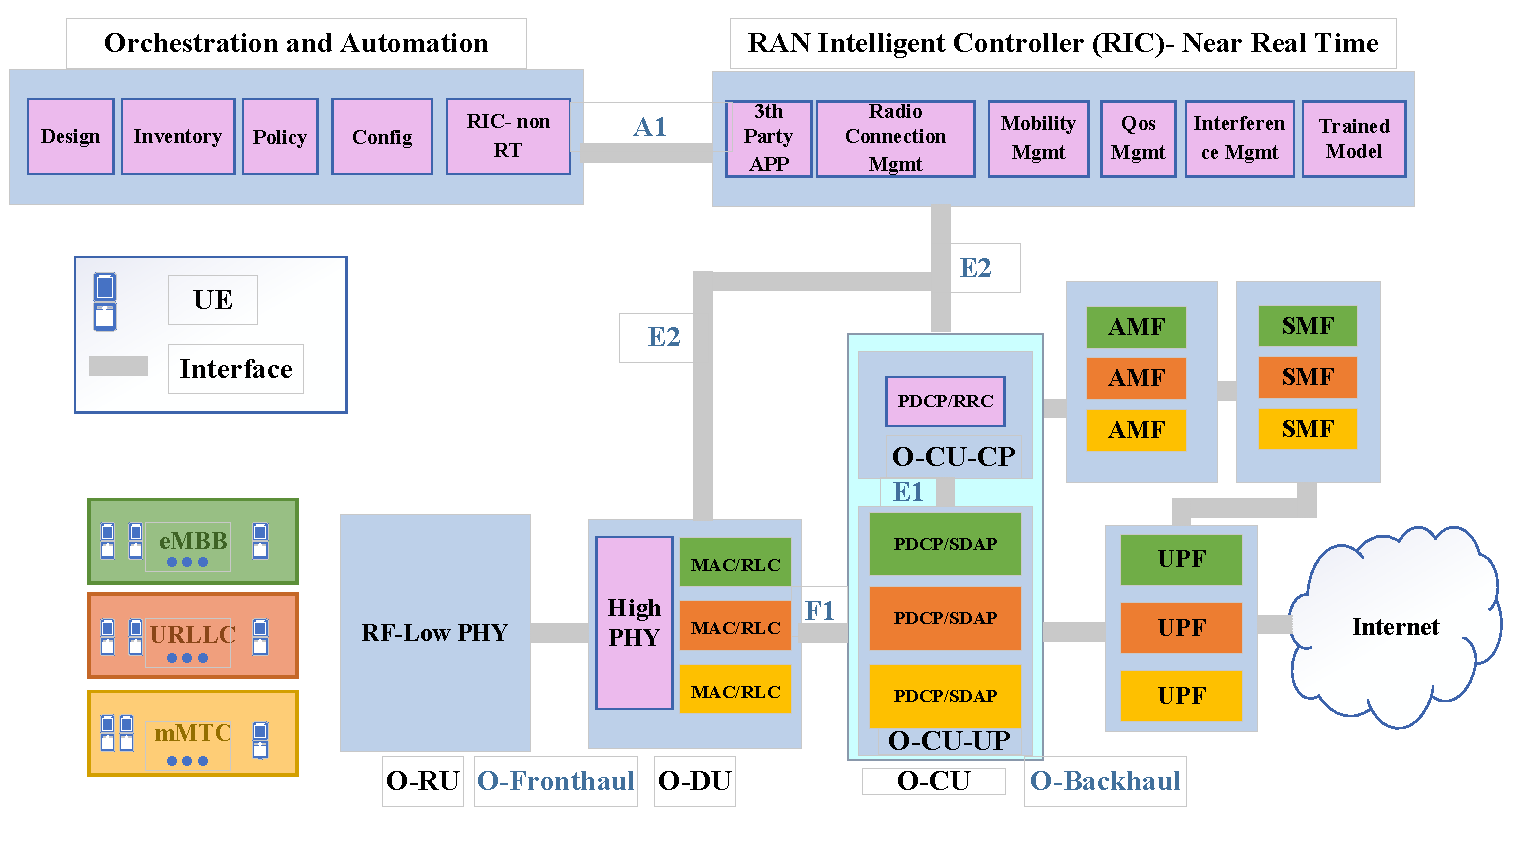
\includegraphics[width=\textwidth]{finalDraw.pdf}
  \caption{Network sliced ORAN system}
  \label{fig:c11}
\end{figure*}

The rest of this paper is organized as follow. The system model and the problem formulation is described 
in Section \ref{systemmodel}. The details of our proposed resource management algorithm is 
introduced in Seection \ref{proAlg}. In Section \ref{NE}, numerical results are provided to evaluate the performance of the proposed algorithm. Section \ref{conc}, concludes the whole paper.

\section{System Model and Problem Formulation}\label{systemmodel}

In this section, we describe the downlink system in O-RAN slicing as depicted in Figure \ref{fig:c11}. 
Here, firstly, we present the system model. Then, we obtain achievable data rates, power of O-RU and the fronthaul capacity for the downlink (DL) of the ORAN system. Afterward, we discuss about the mean delay and the power of VNFs.
Finally, the main problem is expressed.
\subsection{System Model}
Suppose we have three service types includes mMTC, eMBB and URLLC which support different applications.

Assume we have $S_1$, $S_2$ and $S_3$ different applications for the first, second and third service type, respectively ($S = S_1 + S_2 + S_3$).
So, we have $S$ preallocated slices serving these $S$ services; There are $S_1$ slices for the first service type (eMBB), $S_2$ slices for the second service type (URLLC) and $S_3$ slices for the third service type (mMTC). So each service request $s$ served by its corresponding slice.

Each Service $s_j\in \{1,2,...,S_j\} $ consists of $U_{s}$ request from the 
single-antenna UEs which require certain QoS to be able to use the requested program($j \in \{1,2,3\}$ indicate service type).
There are different application request which fall into one of these service categories. Each application request requires specific QoS. Based on the request for the application and QoS, UE may be admitted and allocated to the resources.
Each slice $s_j \in \{1,2,...,S_j \}$, $j \in \{1,2\}$ consists of  preallocated virtual resource blocks that are mapped to the Physical Resource Blocks (PRBs), $M_s^{d}$ VNFs for the processing of O-DU, $M_s^{c}$ VNFs for the processing of O-CU-UP and $M_s^{u}$ VNFs for the processing of UPF.

All $K$ PRBs can be assigned to the all UE in each service.
Also, each VNF instance is running on the virtual machine (VM) that are using resources from the data centers. Each VM, requires enough resources of CPU, memory, storage and network bandwidth.

In addition, there are $R$ multi-antenna O-RU that are shared between slices. Each O-RU $r \in \{1,2,...,R \}$
has $J$ antenna for transmitting and receiving data.
Also $\mathcal{R} = \{ r | r\in 1,2,...,R \}$ depicts the set of O-RUs.
Moreover, all O-RUs, have access to the all PRBs.
%Coordinated multipoint (CoMP) system is considered here. 
\subsection{The Achievable Rate}
The SNR of $i^{th}$ UE served at slice $s$ on PRB $k$ is obtained from
\begin{equation}\label{eq1}
\rho_{r,u(s,i)}^{k} =  \frac{|p_{r,u(s,i)}^{k}{\bold{h}_{r,u(s,i)}^{H \: k}} \bold{w}_{r,u(s,i)}^{k}|^2}{BN_0 + I_{r,u(s,i)}^{k}},
\end{equation} 
where $p_{r,u(s,i)}^{k}$ represents the transmission power from O-RU $r$ to $i^{th}$ UE served at slice $s$ on PRB $k$. 
${\bold{h}_{r,u(s,i)}^{k}} \in \mathbb{C}^{J}$ is the vector of channel gain of a wireless link from 
$r^{th}$ O-RU to the $i^{th}$ UE in $s^{th}$ slice. In addition, $\bold{w}_{r,u(s,i)}^{k} \in \mathbb{C}^{J}$ depicts the  transmit beamforming vector from $r^{th}$ O-RU to the $i^{th}$ UE in $s^{th}$ slice that is the zero forcing beamforming vector to minimize the interference which is indicated as below
\begin{equation}
\bold{w}_{r,u(s,i)}^{k} = {\bold{h}_{r,u(s,i)}^{k}}({\bold{h}_{r,u(s,i)}^{H \: k}} {\bold{h}_{r,u(s,i)}^{k}})^{-1}
\end{equation}
Moreover, $g_{u(s,i)}^r \in \{0,1\}$ is the binary variable that illustrates whether O-RU $r$ served the $i^{th}$ UE that is allocated to $s^{th}$ slice or not. 
%Here, it is assumed that each UE is served by the nearest o-RU
Also, $BN_0$ denotes the power of Gaussian additive noise, and $I_{r,u(s,i)}^{k}$ is the power of interfering signals represented as follow

\begin{equation}\label{eqI}
\begin{split}
I_{r,u(s,i)}^{k} &=
 \underbrace{\sum_{\substack{l=1 \\ l\neq i}}^{{U}_{s}} \gamma_{1}  p_{u(s,l)}^{k}\sum_{\substack{r'=1 \\ r'\neq r}}^{R}|{\bold{h}_{r',u(s,i)}^{H \: k}} \bold{w}_{r',u(s,l)}^{k} g_{u(s,l)}^{r'}|^2}_{\text{(intra-slice interference)}}\\
&+ \underbrace{\sum_{\substack{n = 1 \\ n\neq s}}^{S}\sum_{l=1}^{{U}_s} \gamma_{2}  p_{u(n,l)}^{k}\sum_{\substack{r'=1 \\ r'\neq r}}^{R}|{\bold{h}_{r',u(s,i)}^{H \: k}} \bold{w}_{r',u(n,l)}^{k} g_{u(n,l)}^{r'}|^2}_{\text{(inter-slice interference)}}\\
&+\underbrace{  \sum_{j=1}^{{R}} {\sigma_q}_{r_j}^2 |\boldsymbol{h}_{r,{u(s,i)}}|^2 }_{\text{(Quantization Noise Interference)}}
\end{split}
\end{equation}
where $\gamma_{1} = e^{k}_{u(s,i)}e^{k}_{u(s,l)}$ and $\gamma_{2} = e^{k}_{u(s,i)}e^{k}_{u(n,l)}$.\newline
$e^{k}_{u(s,i)}$ is the binary variable to show whether the $k^{th}$ PRB is allocated to the UE $i$ in slice $s$, assigned to $r^{th}$ o-RU.

To obtain SNR as formulated in \eqref{eq1}, let $y_{u(s,i)} $ be the received signal user $i$ in $s^{th}$ service
\begin{equation}\label{eq2}
\textstyle y_{u(s,i)} = \sum_{r = 1}^{R}\sum_{k=1}^{K_s} \boldsymbol{h}^{H \: k}_{r,u(s,i)} g_{u(s,i)}^r e^k_{r,u(s,i)}\mathfrak{y}^k_{r,u(s,i)}+ z_{u(s,i)},
\end{equation}
%\boldsymbol{w}^k_{r,u(s,i)}p^k_{r,u(s,i)}
where $\mathfrak{y}^k_{r,u(s,i)} =\boldsymbol{w}^k_{r,u(s,i)}{p^{k \: \frac{1}{2}}_{r,u(s,i)}} x_{u(s,i)}+ \boldsymbol{q}_{r}$
and $ x_{u(s,i)}$ depicts the transmitted symbol vector of UE $i$ in $s^{th}$ set of service,  $z_{u(s,i)}$ is the additive Gaussian noise $z_{u(s,i)} \backsim \mathcal{N}(0,N_0)$ and $N_0$ is the noise power.
In addition, $\boldsymbol{q}_{r} \in \mathbb{C}^{J }  $ indicates the quantization noise, which is made from signal compression in O-DU.

The achievable data rate for the $i^{th}$ UE request in the $s_{1}^{th}$ application of service type 1 (eMBB) can be written as $\mathcal{R}_{u(s_1,i)}$ that is formulated as below.
\begin{equation}\label{eq3}
\begin{split}
\mathcal{{R}}_{r,u(s_1,i)}^{k} &=  B \log_2({1+ \rho_{r,u(s_1,i)}^{k}}) ,\\
\mathcal{R}_{u(s_1,i)}^{r} &= \sum_{k=1}^{K} B \log_2({1+ \rho_{r,u(s_1,i)}^{k}} e^k_{r,u(s_1,i)}),\\
\mathcal{R}_{u(s_1,i)} &= \sum_{r=1}^{R}\mathcal{R}_{u(s_1,i)}^{r} g^r_{u(s_1,i)}
\end{split}
\end{equation}
where $B$ is the bandwidth of system. 
$\mathcal{R}_{u(s_1,i)}^{r}$ is the achievable rate of each RU $r$ to UE $i$ in slice $s_1$.
Since the blocklength in URLLC and mMTC is finite, the achievable data rate for the $i^{th}$ UE request in the $s_{j}^{th}$ ( $j \in \{2,3\}$) application of service type 2 (URLLC) and 3 (mMTC) is not achieved from Shannon Capacity formula. So, for the short packet transmission the achievable data rate is approximated from follow
\begin{equation}\label{eq11}
\begin{split}
\mathcal{{R}}_{r,u(s_j,i)}^{k} &= B \log_2({1+ \rho_{r,u(s_j,i)}^{k}} - \zeta_{u(s_j,i)}^{k}){e}_{u(s_j,i)}^{k},\\
\mathcal{R}_{u(s_j,i)}^{r} &= \sum_{k=1}^{K} B (\log_2({1+ \rho_{u(s_2,i)}^{k}})- \zeta_{u(s_j,i)}^{k}){e}_{u(s_j,i)}^{k}\\
\mathcal{R}_{u(s_j,i)} &= \sum_{r=1}^{R}\mathcal{R}_{u(s_j,i)}^{r} g^r_{u(s_j,i)}
\end{split}
\end{equation}
Where $j \in \{1,2\}$. Also we have
\begin{equation}\label{shortPacket}
 \zeta_{u(s_j,i)}^{k} = log_2({e})Q^{-1}(\epsilon) \sqrt{\frac{\mathfrak{C}_{u(s_j,i)}^{k}}{N_{u(s_j,i)}^{k}}})
\end{equation}
Where, $\epsilon $ is the transmission probability, $Q^{-1}$ is the inverse of Q- function (Gaussian),
$\mathfrak{C}_{u(s_j,i)}^{k} = 1 - \frac{1}{(1+\rho_{u(s_j,i)}^{k})^2}$ depicts the channel dispersion of UE  $i$ at slice $s_j$, experiencing PRB $k$ and
$N_{u(s_j,i)}^{k}$ represents the blocklength of it. 
$\mathcal{R}_{u(s_j,i)}^{e,r}$ is the achievable rate of each O-RU $r$ to UE $i$ in slice $s_j$.

If we replace $p_{u(s,l)}^{k}$ and $p_{u(n,l)}^{k}$ in \eqref{eqI} by $P_{max}$, an upper bound $\bar{I}_{r,u(s,i)}^{k}$ is obtained for $I_{r,u(s,i)}^{k}$. Therefore, $\bar{\mathcal{R}}_{u_{(s,i)}} \forall s , \forall i$ is derived by using $\bar{I}_{r,u(s,i)}^{k}$ instead of $I_{r,u(s,i)}^{k}$ in  \eqref{eq11} and \eqref{eq3}.
\subsection{Power of O-RU and Fronthaul Capacity}
Let $P_r$ denote the power of transmitted signal from the $r^{th}$ O-RU to UEs served by it.
From \eqref{eq2}, we have,
\begin{equation}\label{pr}
P_r = \sum_{s=1}^{S}\sum_{k=1}^{K_s}\sum_{i=1}^{U_s}|\bold{w}_{r,u(s,i)}^{k}|^2 p_{r,u(s,i)}^{k} g_{u(s,i)}^r e^k_{r,u(s,i)}+ \sigma_{q_r}^2.
\end{equation}
Since we have fiber link between O-RU and O-DU, the rate of users on the fronthual link between O-DU and the $r^{th}$ O-RU  is formulated as
%\cite{simeone2016cloud, 1111}
\begin{equation}\label{cr}
C_{r} = \log{(1+ \frac{\sum_{s=1}^{S}\sum_{k=1}^{K_s}\sum_{i=1}^{U_s}|\bold{w}_{r,u(s,i)}^{k}|^2 \mathcal{\alpha}^k_{r,u(s,i)} }{ \sigma_{q_{r}}^2})},
\end{equation}
Where, $\mathcal{\alpha}^k_{r,u(s,i)}= p_{r,u(s,i)}^{k} g_{u(s,i)}^r e^k_{r,u(s,i)}$ and $\sigma_{q_{r}}^2$ is the power of quantization noise.
\subsection{Mean Delay}
In this part, the end to end mean delay for a service is obtained.
Suppose the mean total delay is depicted as $T_{tot}$.
\begin{equation}
\begin{split}
T_{tot} &=  T_{process} + T_{transmission} + T_{propagation}\\
T_{process} &=  T_{RU} + T_{DU} + T_{CU} + T_{UPF}\\
T_{transmission} &= T_{front} + T_{mid} + T_{back} + T_{trans2net} \\
T_{propagation} &= T_{front} + T_{mid} + T_{back} + T_{trans2net} \\
\end{split}
\end{equation}
%T_{tot} = T_{RU} + T_{front} + T_{DU} + T_{mid} + T_{CU} + T_{back} + T_{core} + T_{trans2net}
Total delay is sum of processing delay, transmission delay and propagation delay. 
The propagation delay is the time takes for a signal to reach to its destination. So it has a constant value based on the length of fiber link ($T = L/c$, where $L$ is the length of link and c is the speed of signal).
Also, the transmission delay is the amount of time required to push all the packets into the fiber link. 
($T = \frac{\alpha}{R}$ Where, $R$ is the rate of transmission in each link and $\alpha$ is the mean arrival data rate of the each link which is constant in this model.)
Here we assume the value of propagation delay and transmission is negligible compared to the rest.
\begin{equation}
T_{tot} \approx T_{process}
\end{equation}
\subsubsection{Processing Delay}
Assume the packet arrival of UEs follows a Poisson process with arrival rate $\lambda_{u(s,i)}$ for the $i^{th}$ UE of the $s^{th}$ slice.
Therefore, the mean arrival data rate of the $s^{th}$ slice in the UPF layer is $\alpha_{s}^U = \sum_{u=1}^{U_s}\lambda_{u(s,i)}$.
Assume the mean arrival data rate of the UPF layer for slice $s$ ($\alpha_{s}^U$) is approximately equal to the mean arrival data rate of the O-CU-UP layer ($\alpha_{s}^C$) and O-DU ($\alpha_{s}^D$). so $\alpha_{s} =\alpha_{s}^U \approx \alpha_{s}^C \approx \alpha_{s}^D$. since, by using Burke’s Theorem, the mean arrival data rate of the second and third layer which are processed in the first layer is still Poisson with rate $\alpha_{s}$.
It is assumed that there are load balancers in each layer for each service to divide the incoming traffic to VNFs equally. %\cite{frdl,luong2018novel,luong2018novel1}.
Suppose the baseband processing of each VNF is depicted as M/M/1 processing queue.
Each packet is processed by one of the VNFs of a slice. So, the mean delay for the $s^{th}$ slice in the first and the second layer, modeled as M/M/1 queue, is formulated as follow, respectively
\begin{equation}
\begin{split}
T_{DU}^{s} &= \frac{1}{\mu_s^d - \alpha_{s}/{M_s^{d}}},\\
T_{CU}^{s} &= \frac{1}{\mu_s^c - \alpha_{s}/{M_s^{c}}}\\
T_{UPF}^{s} &= \frac{1}{\mu_s^u - \alpha_{s}/{M_s^{u}}}\\
\end{split}
\end{equation}
Where $M_s^{d}$, $M_s^{c}$ and 
$M_s^{u}$ are the variables that depict the sum of VNFs in O-DU, O-CU-UP and UPF, respectively. 
Moreover, $1/\mu_s^d$, $1/\mu_s^c$ and $1/\mu_s^u$ are the mean service time of the O-DU, O-CU and the UPF layers respectively.
Besides, $\alpha_{s}$ is the  arrival rate which is divided
by load balancer before arriving to the VNFs. The arrival rate of each VNF in each layer for each slice 
$s$ is $\alpha_{s}/{M_s^{i}}$ $ i \in \{d,c, u\}$.

In addition, $T_{RU}^{u(s,i)}$ is the mean transmission delay of $i^{th}$ UE in $s^{th}$ service on the wireless link.
 The arrival data rate of wireless link for each UE i in service s is $\lambda_{u(s,i)}$
As a result we have, $\sum_{i = 1}^{U_s} \lambda_{u(s,i)} = \alpha_s$.
Moreover, The service time of transmission queue for UE $i$ requesting service $s$ has
an exponential distribution with mean $1/R_{u(s,i)}$ and can be modeled as a M/M/1 queue.
 
Therefore, the mean delay of the transmission layer for UE $i$ in slice $s$ is
\begin{equation}
 T_{RU}^{u(s,i)} = \frac{1}{R_{u(s,i)} - \lambda_{u(s,i)}};
\end{equation}

So the mean processing delay for each UE $i$ in slice $s$ is 
\begin{equation}
T_{process}^{u(s,i)} =  T_{RU}^{u(s,i)} + T_{DU}^{s} + T_{CU}^{s} + T_{UPF}^{s}
\end{equation}
Hence, $T_{tot}^{u(s,i)} \approx T_{process}^{u(s,i)} $
%Furthermore, the mean arrival data rate of the each link ($\textstyle \alpha_{s}^i$ , $i \in \{RU,DU,CU,UPF\}$) is approximately equal to others ($\textstyle \alpha_{s} \approx \alpha_{s}^i$ , $i \in \{RU,DU,CU,UPF\}$).  
\subsection{VNF Power}
Assume the power consumption of baseband processing at each DC $d$ that is connected to VNFs of a slice $s$ is depicted as
$\phi_{s}$. So the total power of the system for all active DCs that are connected to slices can be represented as
\begin{equation*}
\textstyle \phi_{tot} = \sum_{s=1}^{S}\phi_{s}.
\end{equation*}
Where, $\phi_{s}$ is obtained from below
\begin{equation}
\phi_{s} = M_s^u \phi_s^u + M_s^c \phi_s^c+ M_s^d \phi_s^d
\end{equation}
Moreover, $\phi_s^u$, $\phi_s^c$ and $\phi_s^d$ are the static cost of energy in UPF, O-CU and O-DU, respectively. 
\subsection{Problem Statement}
Suppose each slice $s$ has priority factor $\delta_s$ where $\sum_{s=1}^S \delta_s =1$.
The optimization problem is formulated as follow.
The aim of this paper is to maximize the sum rate of all UEs with the presence of constraints which is written as follow,
\begin{subequations}\label{problem}
\begin{alignat}{4}
\max\limits_{\boldsymbol{P}, \boldsymbol{E}, \boldsymbol{M}, \boldsymbol{G} }   \quad &  \sum_{s=1}^{S}\sum_{i=1}^{U_s}\delta_s \bar{\mathcal{R}}_{u_{(s,i)}} \ \\
\text{subject to} \quad  &  P_r \leq P_{max} \quad \forall r
 \label{c11} \\
&p_{r,u(s,i)}^{k}  \geq 0  \quad \forall i,\forall r,\forall s, \forall k,\label{c12} \\
&\bar{\mathcal{R}}_{u_{(s_j,i)}} \geq \mathcal{R}_{min}^{s_j} \quad \forall s, j \in \{1,2,3\}, \label{c13} \\
%&\mathcal{R}_{u_{(s_2,i)}}^u \geq  \mathcal{R}_{min}^{s_2,u} \quad \forall s_2, \label{c14} \\
& C^r \leq C_{max}^r \quad \forall r, \label{c15}\\ 
&T_{tot}^{u(s,i)}  \leq T_{max}^{s} \quad \forall i,\forall s,\label{c16} \\
& \mu_s \geq \alpha_s/M_s \quad \forall s,\label{c16-1} \\
& \bar{\mathcal{R}}_{u_{(s,i)}} \geq {\lambda}_{u_{(s,i)}} \quad \forall i,\forall s,\label{c16-2} \\
& 0 \leq M_s \leq M^{max}  \quad \forall s,\label{c16-3}\\
%& P_r\{E_1, E_2, E_3, E_4\} \leq \epsilon_s \quad \forall s_2, \label{c166}\\
& \sum_{r}g^r_{u(s,i)} = 1  \quad \forall s,\forall i, \label{c17}  \\
& \sum_{k =1}^{K_s} g^r_{u(s,i)} e^{k}_{r,u(s,i)} \geq 1  \quad \forall s,\forall i ,\forall r \label{c18-1} \\
& \sum_{s =1}^{S}\sum_{i=1}^{U_s}g^r_{u(s,i)} e^{k}_{r,u(s,i)} \leq 1  \quad \forall s,\forall i ,\forall r \label{c18} \\
& \phi_{tot}  \leq \phi_{max}, \label{c19} \\
& g^r_{u(s,i)} \in \{0,1\} \quad \forall s,\forall i, \label{c20}  \\
& e^k_{r,u(s,i)} \in \{0,1\} \quad \forall s,\forall i, \label{c21}  
\end{alignat}
\label{constraints}
\end{subequations}
where $\boldsymbol{P} =[p_{r,u(s,i)}^{k}] \:\: \forall s , \forall i, \forall r, \forall k $, is the matrix of power for UEs, $\boldsymbol{E} =[e_{r,u(s,i)}^k] \:\: \forall s , \forall i, \forall r, \forall k$ indicate the binary variable for PRB association. Moreover, $\boldsymbol{G} =[g_{u(s,i)}^r] \:\: \forall s , \forall i, \forall r$ is a binary variable for O-RU association. Furthermore, $M = [M_s^d, M_s^c, M_s^u] \:\: \forall s$ is the matrix that shown the number of VNFs in each layer of slice.
\eqref{c11}, and \eqref{c12}, indicate that the power of each RU do not exceed the maximum power, and the power of each UE is a positive integer value, respectively. 
Also \eqref{c13} shows that the rate of each UE requesting eMBB, URLLC and mMTC is more than a threshold, respectively.
\eqref{c15} and \eqref{c16} expressed the limited capacity of the fronthaul link, and the limited delay of receiving signal, respectively.
\eqref{c16-1} and \eqref{c16-2} denoted the stability of the M/M/1 queue model.
\eqref{c16-3} restricted the number of VNF in each slice due to the limited resources.
%\eqref{c16} is a reliability condition that the delay in each layer should be less than threshold.
\eqref{c17} and \eqref{c18-1} guarantee that O-RU and PRB is associated to the UE, respectively.
Also, \eqref{c18} ensure that each PRB can not be assigned to more than one UE associated to the same O-RU.
In addition, \eqref{c19} indicate that the static cost of energy of VNFs in each slice do not exceed from the threshold. 
Moreover, \eqref{c20} and \eqref{c21} depict that $\boldsymbol{E}$ and $\boldsymbol{G}$ are matrix of binary variables.
\section{Proposed Algorithm Scheme}\label{proAlg}
In this section, we first apply some simplifications to the system; Solving problem \eqref{problem} is complicated due to the fact that this problem is 
a non-convex problem and it is a 
mixed integer non-linear problem (MINLP) with a binary variable and an integer variable. 
In the following, we apply the simplifications to reformulate MINL parts and use iterative heuristic algorithm to solve the reformulated problem.
We solve this problem in two level iteratively until it converges; In the first level,
parameters ($\boldsymbol{P}, \boldsymbol{E}, \boldsymbol{M}$) are obtained by relaxing and reformulating parameters and turn it to convex problem; Afterward we solve it by dual optimization problem.
In the second level, finding optimal O-RU association ($ \boldsymbol{G}$) is concerned with the fixed parameter of power, PRB allocation and number of VNFs.   
We repeat this procedure until the algorithm converges.
\subsection{Sub-Problem 1}\label{sub1}
Suppose that $\boldsymbol{G}$ is fixed, we want to obtain $\boldsymbol{P}, \boldsymbol{E}$ and $\boldsymbol{M}$.
Here, we first simplify and relax the parameters to convexify the problem.

As we mentioned before, by replacing $p_{u(s,l)}^{k}$ and $p_{u(n,l)}^{k}$ in \eqref{eqI} by $P_{max}$, an upper bound $\bar{I}_{r,u(s,i)}^{k}$ for $I_{r,u(s,i)}^{k}$, the lower bound $\bar{\rho}_{u(s,i)}^{k}$ 
for $\rho_{u(s,i)}^{k}$ 
and the lower bound $\bar{\mathcal{R}}_{u_{(s,i)}} \forall s , \forall i$ for  ${\mathcal{R}}_{u_{(s,i)}}$ is obtained by replacing with $I_{r,u(s,i)}^{k}$ $\bar{I}_{r,u(s,i)}^{k}$ in  \eqref{eq11} and \eqref{eq3} and make them concave.

Suppose $\hat{\rho}_{r,u(s,i)}^{k} =  \frac{|P_{max}{\bold{h}_{r,u(s,i)}^{H \: k}} \bold{w}_{r,u(s,i)}^{k} g_{u(s,i)}^r|^2}{BN_0}$. 
To convexify \eqref{eq11} (for the short packet transmission), we replace ${\rho}_{r,u(s,i)}^{k}$ with $\hat{\rho}_{r,u(s,i)}^{k}$ in \eqref{shortPacket}. So, a lower bound for \eqref{eq11} is given that is a concave function.
\begin{equation}
\begin{split}
\bar{\mathcal{R}}_{u(s_j,i)}^{r} &= \sum_{k=1}^{K_{s_j}} B (\log_2({1+ \bar{\rho}_{u(s_2,i)}^{k}})- \hat{\zeta}_{u(s_j,i)}^{k}){e}_{u(s_j,i)}^{k}\\
\bar{\mathcal{R}}_{u(s_j,i)} &= \sum_{r=1}^{R}\bar{\mathcal{R}}_{u(s_j,i)}^{r}\\ 
 \hat{\zeta}_{u(s_j,i)}^{k} =& log_2({e})Q^{-1}(\epsilon) \sqrt{\frac{\hat{\mathfrak{C}}_{u(s_j,i)}^{k}}{N_{u(s_j,i)}^{k}}})\\
 \hat{\mathfrak{C}}_{u(s_j,i)}^{k} =& 1 - \frac{1}{(1+\hat{\rho}_{u(s_j,i)}^{k})^2}\\
\end{split}
\end{equation}
Consider UPF, O-CU and O-DU have the same processor (for simplification), so we have $\mu_s = \mu_s^u \approx \mu_s^c \approx \mu_s^d $. Moreover, as mentioned before,
the mean arrival data rate of the UPF layer for a service $s$ ($\alpha_{s}^U$) is approximately equal to the mean arrival data rate of the O-CU-UP layer ($\alpha_{s}^C$) and O-DU ($\alpha_{s}^D$). so $\alpha_{s} =\alpha_{s}^U \approx \alpha_{s}^C \approx \alpha_{s}^D$. 
So the given assumption leads to have same energy for each layer $\phi_s^u = \phi_s^c =\phi_s^d $.
As a result of these assumption, for simplicity, we can assume that $M_s = M_s^u = M_s^c = M_s^d $
Using the above assumption, we have $T_{DU}^{s} = T_{CU}^{s} = T_{UPF}^{s}$ 
\begin{equation}
\begin{split}
T_{process}^{s} &=  T_{RU}^{s} + T_{DU}^{s} + T_{CU}^{s} + T_{UPF}^{s} \\
T_{process}^{s} &=  T_{RU}^{s} + 3\times T_{DU}^{s}.
\end{split}
\end{equation}
\begin{lemma}
In problem \eqref{problem}, the constraint \eqref{c16} can be reformulated as below
$ \forall i,\forall s$
\begin{equation}
\begin{split}
&T_{max}^s \geq\frac{1}{R_{u(s,i)} - \lambda_{u(s,i)}} + \frac{3}{\mu_s - \alpha_{s}/{M_s}}  \\
&M_s \geq \frac{\alpha_s(T_{max}^s R_{u(s,i)}-T_{max}^s\lambda_{u(s,i)} -1)}{(T_{max}^s\mu_s-3)(R_{u(s,i)}-\lambda_{u(s,i)}) - \mu_s }\\
\end{split}
\end{equation}
Also from equation \eqref{c19}, \eqref{c16-1} and \eqref{c16-3} we have
\begin{equation}
0\leq M_s \leq \min\{M^{max}, \alpha_s/\mu_s, \phi_{max}/{3\phi_s}\}
\end{equation}
We denote $ \mathfrak{M}_s= \min\{M^{max}, \alpha_s/\mu_s, \phi_{max}/{3\phi_s}\}$.
Thus, if we restrict \eqref{c16} to equality we have
\begin{equation}\label{eqDelay}
0\leq \frac{\alpha_s(T_{max}^s R_{u(s,i)}-T_{max}^s\lambda_{u(s,i)} -1)}{(T_{max}^s\mu_s-3)(R_{u(s,i)}-\lambda_{u(s,i)}) - \mu_s } \leq \mathfrak{M}_s
\end{equation}
In \eqref{eqDelay}, $0\leq \frac{\alpha_s(T_{max}^s R_{u(s,i)}-T_{max}^s\lambda_{u(s,i)} -1)}{(T_{max}^s\mu_s-3)(R_{u(s,i)}-\lambda_{u(s,i)}) - \mu_s }$ is established due to the fact that 
the numerator and the denominator will both have same sign. Using \eqref{c16-2},
in numerator, $\alpha_s \geq 0$, $ R_{u(s,i)}-\lambda_{u(s,i)} \geq 0$ and to simplify the problem, assume 
$(R_{u(s,i)}-\lambda_{u(s,i)})T_{max}^s \geq 1$ since the order of $T_{max}^s$ is about milli second and the difference between achievable rate and packet rate can be more than $1/T_{max}^s$.
Therefore, we restrict constraint \eqref{c16-2} to $R_{u(s,i)} \geq \lambda_{u(s,i)} + 1/T_{max}^s$.
So the numerator is positive.
In denominator, it can be said approximately that $(T_{max}^s\mu_s)(R_{u(s,i)}-\lambda_{u(s,i)}) - \mu_s \geq 0 $, since, $(R_{u(s,i)}-\lambda_{u(s,i)}) \geq 1/T_{max}^s$ as mentioned above.
Therefore, we just need to have constraint below
\begin{equation}\label{constraint16}
\frac{\alpha_s(T_{max}^s R_{u(s,i)}-T_{max}^s\lambda_{u(s,i)} -1)}{(T_{max}^s\mu_s-3)(R_{u(s,i)}-\lambda_{u(s,i)}) - \mu_s } \leq \mathfrak{M}_s
\end{equation}
So by reformulating the equation \eqref{constraint16}, we have a new constraint $\forall i, \forall s$ as below,
\begin{equation}\label{RM}
\begin{split}
\mathcal{R}_{u(s,i)} &\geq \frac{\mathfrak{M}_s ((T_{max}^s\mu_s-3)\lambda_{u(s,i)} + \mu_s) - \alpha_s(T_{max}^s\lambda_{u(s,i)} +1) }{\mathfrak{M}_s (T_{max}^s\mu_s-3)-\alpha_s T_{max}^s},\\
\varpi_{u(s,i)} &= \frac{\mathfrak{M}_s ((T_{max}^s\mu_s-3)\lambda_{u(s,i)} + \mu_s) - \alpha_s(T_{max}^s\lambda_{u(s,i)} +1) }{\mathfrak{M}_s (T_{max}^s\mu_s-3)-\alpha_s T_{max}^s},\\
\mathcal{R}_{u(s,i)} &\geq \varpi_{u(s,i)}. \\
\end{split}
\end{equation}
In addition, we denote $\mathtt{M}_{u(s,i)} = \frac{\alpha_s(T_{max}^s R_{u(s,i)}-T_{max}^s\lambda_{u(s,i)} -1)}{(T_{max}^s\mu_s-3)(R_{u(s,i)}-\lambda_{u(s,i)}) - \mu_s }$.
So we have,
\begin{equation}
M_s = \max\{\mathtt{M}_{u(s,i)} | i \in 1,2,..., U_s\} \quad \forall s .
\end{equation}
\end{lemma}
Despite simplifying the problem \eqref{problem}, it is still non-convex and hard to be solved.
So the simplest approach is to relax $\mathbf{E}$ into continuous value $e_{r,u(s,i)}^k \in [0,1] \:\: \forall s , \forall i ,\forall r, \forall k$
Furthermore, the problem can  be solved using the Lagrangian function and iterative algorithm.

In order to make \eqref{problem} as a standard form of a convex optimization problem, it is required to change the variable of equations \eqref{cr} to $P_r = \sigma_{q_r}^2\times 2^{C^r}$ so the constraint 
\eqref{c15} is changed to
 $P_r \leq \sigma_{q_r}^2\times 2^{C^r_{max}}$.
The combination of equations \eqref{c13} and \eqref{c15} leads to the following equation
\begin{equation}
\begin{split}
\zeta_{r}&= min\{P_{max}, \sigma_{q_r}^2\times 2^{C^r_{max}} \}, \\
P_r &\leq  \zeta_{r}.\\
\end{split}
\end{equation} 
Moreover, the combination of equations \eqref{c13}, \eqref{c16-2} and \eqref{RM} leads to the following equation
\begin{equation}\label{RConstr}
\begin{split}
\eta_{u_{(s,i)}}&= max\{\mathcal{R}_{u_{(s,i)}}^{max}, \lambda_{u_{(s,i)}}+1/T^s_{max}, \varpi_{u(s,i)} \}, \\
\mathcal{\bar{R}}_{u_{(s,i)}} &\geq  \eta_{u_{(s,i)}}.\\
\end{split}
\end{equation}
Assume $\boldsymbol{\mathfrak{v}}$, $\boldsymbol{\mathfrak{m}}$, $\boldsymbol{\mathfrak{h}}$, $\boldsymbol{\xi}$, $\boldsymbol{\chi}$ and $\boldsymbol{ \kappa}$ are the matrix of Lagrangian multipliers that have non-zero positive elements.

The Lagrangian function is written as follow
\begin{subequations}\label{lagrang}
\begin{alignat}{4}
&\mathcal{L}(\boldsymbol{P},\boldsymbol{E}; \boldsymbol{\mathfrak{v}}, \boldsymbol{\chi}, \boldsymbol{\mathfrak{h}}, \boldsymbol{ \xi}, \boldsymbol{ \kappa}, \boldsymbol{\mathfrak{m}})  = \sum\limits_{s=1}^{S} \sum\limits_{i=1}^{U_s}\delta_s\mathcal{\bar{R}}_{u_{(s,i)}}\\
&+\sum\limits_{s=1}^{S} \sum\limits_{i=1}^{U_s}\mathfrak{h}_{u_{(s,i)}} (\mathcal{\bar{R}}_{u_{(s,i)}}-\eta_{u_{(s,i)}})\\
&-  \sum\limits_{r=1}^{R} \mathfrak{m}_{r} (P_{r}- \zeta_r)\\
&+  \sum\limits_{s=1}^{S} \sum\limits_{i=1}^{U_s}\sum\limits_{k=1}^{K} \sum\limits_{r=1}^{R}\kappa^k_{r,u(s,i)}  p^k_{r,u(s,i)}\\
&+ \sum\limits_{r=1}^{R}\sum\limits_{s=1}^{S} \sum\limits_{i=1}^{U_s}\chi_{r,u(s,i)}(\sum_{k =1}^{K_s} e^{k}_{r,u(s,i)} -1)\\
&-  \sum\limits_{s=1}^{S} \sum\limits_{i=1}^{U_s}\sum\limits_{k=1}^{K} \sum\limits_{r=1}^{R}\mathfrak{v}^{k}_{r,u(s,i)} (e^{k}_{r,u(s,i)} -1)\\
&+  \sum\limits_{s=1}^{S} \sum\limits_{i=1}^{U_s}\sum\limits_{k=1}^{K} \sum\limits_{r=1}^{R} \xi^{k}_{r,u(s,i)} e^{k}_{r,u(s,i)}.
\end{alignat}
\end{subequations}
\begin{lemma}
By taking derivatives of \eqref{lagrang} (the lagrangian function), with respect to the $\boldsymbol{P}$ and the $\boldsymbol{E}$, these two variables are obtained.
Assume, $e_{r,u(s,i)}^{k} = 1$
\begin{equation}\label{deriveP}
\dfrac{\partial\mathcal{L}}{\partial p_{r,u(s,i)}^{k}} = (\delta_s + \mathfrak{h}_{u_{(s,i)}})\mathfrak{B}_{r,u(s,i)}^{k} + (\kappa^k_{r,u(s,i)} -\mathfrak{m}_{r}\mathfrak{D}_{r,u(s,i)}^{k})=0
\end{equation}
Where
\begin{equation}
\begin{split}
\mathfrak{D}_{r,u(s,i)}^{k} &= |\bold{w}_{r,u(s,i)}^{k}|^2 g_{u(s,i)}^r e^k_{r,u(s,i)}, \\
\mathfrak{B}_{r,u(s,i)}^{k} &= \frac{B |{\bold{h}_{r,u(s,i)}^{H \: k}} \bold{w}_{r,u(s,i)}^{k}|^2 g_{u(s,i)}^r e_{r,u(s,i)}^{k}}{\ln(2)} \mathfrak{S}_{r,u(s,i)}^{k},\\
\mathfrak{S}_{r,u(s,i)}^{k} &= \frac{1}{{|\bold{h}_{r,u(s,i)}^{H \: k}} \bold{w}_{r,u(s,i)}^{k}|^2 \mathfrak{k}_{r,u(s,i)}^{k}+BN_0 + I_{r,u(s,i)}^{k}}.\\
\end{split}
\end{equation}
where $\mathfrak{k}_{r,u(s,i)}^{k} = g_{u(s,i)}^r e_{r,u(s,i)}^{k}p_{r,u(s,i)}^{k}$.
Thus, from equation \eqref{deriveP}, optimal power is obtained and power is allocated.
We denote $ \mathfrak{j}_{r,u(s,i)}^{k} = g_{u(s,i)}^r e_{r,u(s,i)}^{k}$.
\begin{equation}
p_{r,u(s,i)}^{k} = [\frac{(\delta_s + \mathfrak{h}_{u_{(s,i)}})B \mathfrak{j}_{r,u(s,i)}^{k}}{\kappa^k_{r,u(s,i)} -\mathfrak{m}_{r}\mathfrak{D}_{r,u(s,i)}^{k}} -\frac{BN_0 + I_{r,u(s,i)}^{k}}{{|\bold{h}_{r,u(s,i)}^{H \: k}} \bold{w}_{r,u(s,i)}^{k}|^2\mathfrak{j}_{r,u(s,i)}^{k}}]^+.
\end{equation}
Also $[a]^+ = \max(0,a)$.
In addition, PRB assignment is obtained as follow
\begin{equation}\label{deriveE}
\begin{split}
\dfrac{\partial\mathcal{L}}{\partial e_{r,u(s,i)}^{k}} &= \mathcal{\bar{R}}_{r,u(s,i)}^{k}(\delta_s+\mathfrak{h}_{u_{(s,i)}})\\
&- \mathfrak{m}_{r}|\bold{w}_{r,u(s,i)}^{k}|^2 p_{r,u(s,i)}^{k} g_{u(s,i)}^r\\
&+( \xi^{k}_{r,u(s,i)}-\mathfrak{v}^{k}_{r,u(s,i)} +\chi_{r,u(s,i)})=0.\\
\end{split}
\end{equation}
Using KKT conditions, we have
\begin{equation}\label{deriveE1}
e_{r,u(s,i)}^{k}\times (\mathfrak{F}^{k}_{r,u(s,i)} -\mathfrak{v}^{k}_{r,u(s,i)} - \mathfrak{m}_{r}|\bold{w}_{r,u(s,i)}^{k}|^2 p_{r,u(s,i)}^{k} g_{u(s,i)}^r ) = 0.
\end{equation}
Where $\mathfrak{F}^{k}_{r,u(s,i)} =\mathcal{\bar{R}}_{r,u(s,i)}^{k}(\delta_s+\mathfrak{h}_{u_{(s,i)}})+( \xi^{k}_{r,u(s,i)} +\chi_{r,u(s,i)}) $.
Hence, from equation \eqref{deriveE} and \eqref{deriveE1}, PRB assignment is performed as follow.
\begin{equation}
e_{r,u(s,i)}^{k} = 
  \begin{cases}
      1 & u(s,i) = \text{argmax} \mathfrak{F}^{k}_{r,u(s,i)} \forall s, \forall r, \forall k\\
      0 & \text{otherwise}
    \end{cases}
\end{equation}
\end{lemma}
Thus the user in each slice $s$ that have the largest value of $\mathfrak{F}^{k}_{r,u(s,i)}$, should be allocated to the PRB $k$; Due to the fact that just one PRB can be allocated to a UE between those UEs (regardless to the services) that are associated to the same O-RU.
\subsection{Sub-Problem 2}\label{sub2}
After power allocation and PRB assignment, the remaining problem is to assign O-RU to the UE in each service.

Assume $\boldsymbol{P}$ and $\boldsymbol{E}$ are fixed, we want to find $\boldsymbol{G}$.
Next we introduce a greedy algorithm that assign one O-RU to each UE.

\textit{Greedy Algorithm for Non-Comp O-RU Assignment:}
The problem can be reformulated as follow
\begin{subequations}\label{problem2}
\begin{alignat}{4}
\max\limits_{ \boldsymbol{G} }   \quad &  \sum_{s=1}^S\sum_{i=1}^{U_s}\sum_{r=1}^{R} \delta_s g^r_{u(s,i)}\bar{\mathcal{R}}^r_{u_{(s,k)}} \ \\
\text{subject to} \quad  & \sum_{s=1}^{S}\sum_{i=1}^{U_s} g_{u(s,i)}^r \psi_{r,u(s,i)}\leq \mathfrak{t}_r \quad \forall r
 \label{p11} \\
& \sum_{r}g^r_{u(s,i)} = 1  \quad \forall s,\forall i, \label{p12}\\
 & g^r_{u(s,i)} \in \{0,1\} \quad \forall s,\forall i, \label{p13}  
\end{alignat}
\end{subequations}
Where $ \psi_{r,u(s,i)}=\sum_{k=1}^{K_s}|\bold{w}_{r,u(s,i)}^{k}|^2 p_{r,u(s,i)}^{k}  e^k_{r,u(s,i)}$
and $\mathfrak{t}_r = \zeta_r- \sigma_r$
Since we obtained \eqref{RConstr} in \eqref{sub1}, we can ignore this constraint in \eqref{problem2}.
%The problem \eqref{problem2} is an integer linear programming.
%By changing inequality \eqref{p12} to equality ($\sum_{r}g^r_{u(s,i)} = 1$),
The problem \eqref{problem2} is an NP-complete 0-1 multiple knapsack problem.  
We solve this problem using GAAOU which is a greedy algorithm \eqref{alg1} as follow \cite{akccay2007greedy,lee2018dynamic}.
Firstly, we set all variables $g^r_{u(s,i)} = 0, \quad \forall s, \forall i, \forall r$. 
Then we define ${\mathfrak{B}}^{rem}_{u_{(s,i)}} = \mathcal{R}$  $\forall s, \forall i$ and $ \mathfrak{C}_r = \mathfrak{t}_r, \forall r$
as a set of all O-RUs and value of each O-RU, respectively.
Next, we sort all slices based on their priority. 
Afterward, we assign the O-RU that provides the highest achievable rate for each UE (we start from the UEs on the slices with highest priority) on the condition that 
it does not exceed the value of each O-RU (that is a function of maximum power and capacity of O-RU).
If it exceeds the value of O-RU, then O-RU with the next highest achievable rate is selected. 
The complexity of sorting S slices based on their priority is $O(Slog(S))$.
Depict $\mathfrak{N} =  \sum_{s=1}^S\sum_{i=1}^{U_s} 1$. 
The complexity of this algorithm is about $O(Slog(S)) + O(R\times \mathfrak{N})$.
%$O(N\times \mathfrak{N})$
\begin{algorithm}
\caption{Greedy Algorithm for Assignment of O-RU to UEs (GAAOU)}\label{alg1}
\begin{algorithmic}[1]
\State Set $g^r_{u(s,i)} = 0, \quad \forall s, \forall i, \forall r$.\label{31}
\State Set $\mathfrak{C}_r = \mathfrak{t}_r, \forall r$  \label{32}
\State Set ${\mathfrak{B}}^{rem}_{u_{(s,i)}} = \mathcal{R}$  $\forall s, \forall i$
\State Sort slices according to their priority factor ($\delta_s$) in descending order
\For {$s \gets 1$ to $S$}\label{33}
\For {$i \gets 1$ to $U_s$}
\State $RU = 0$
\For {$r \gets 1$ to $R$}
\State Acquire $\mathfrak{G}^r_{u_{(s,i)}} = \bar{\mathcal{R}}^r_{u_{(s,i)}}$
\EndFor
\State \textbf{end for}
\State Obtain $r^* = \text{argmax}_{r\in{\mathfrak{B}}^{rem}_{u_{(s,i)}}} \mathfrak{G}^r_{u_{(s,i)}}$
\While{$RU == 0$}
\If{$\mathfrak{C}_{r^*} \geq \psi_{r^*,u(s,i)}$}
\State Set $g^{r^*}_{u(s,i)} = 1$ 
\State Set  $\mathfrak{C}_{r^*} = \mathfrak{C}_{r^*} - \psi_{{r^*},u(s,i)}$
\State Set $RU = 1$ 
\Else
\State  ${\mathfrak{B}}^{rem}_{u_{(s,i)}} = \mathcal{R} \setminus \{{r^*}\} $
\EndIf
\State \textbf{end if}
\EndWhile
\State \textbf{end while}
\EndFor
\State \textbf{end for}
\EndFor
\State \textbf{end for} \label{34}
\end{algorithmic}
\end{algorithm} 
\subsection{Iterative Proposed Algorithm}
In \eqref{sub1} and \eqref{sub2}, the details of solving each sub-problem are depicted. 
Here, the iterative algorithm for the whole problem is demonstrated.
Firstly, we fixed $\boldsymbol{G}$, then $\boldsymbol{P}$ and $\boldsymbol{E}$ is achieved using Lagrangian method.  
Afterward, $\boldsymbol{G}$ is updated using GAAOU algorithm. This process is repeated until it converges. 
The whole algorithm is depicted as follow (Algorithm \eqref{alg2}).
 \begin{algorithm}
\caption{Iterative Algorithm for Power Allocation, PRB, VNF and O-RU Association (IAPPVO)}\label{alg2}
\begin{algorithmic}[1]
\State  Set the maximum number of iterations ${Iter}_{max}$, convergence condition $\epsilon > 0$ \label{a21}
\State  Assign Users to O-RU randomly (Initialize $\boldsymbol{G}$) \label{a22}
\For {$i \gets 1$ to $Iter_{max}$}\label{23}
\State Acquire $\boldsymbol{P}^{(i)}$, $\boldsymbol{E}^{(i)}$ and $\boldsymbol{M}^{(i)}$ using Lagrangian function and sub-gradient method based on \eqref{sub1}
\State Update $\boldsymbol{G}^{(i)}$   based on algorithm GAAOU \eqref{alg1} in  \eqref{sub2}
\If {the algorithm converged with the tolerence of $\epsilon$}
\State Break
\Else 
\State Continue the algorithm  
\EndIf
\State \textbf{end if}
\EndFor
\State \textbf{end for} \label{24}
\end{algorithmic}
\end{algorithm}
\section{Numerical Results}\label{NE}
In this section, numerical results for the problem are depicted to evaluate the performance of the algorithms. We consider three network slice, one for eMBB, and two another for URLLC and mMtc.
Assume we have six 4-antenna O-RU (MISO), are located in a cell with a diameter of 500 meters. We consider 25 PRB
in the network.
The maximum number of VNF for each slice is 20 and the mean arrival rate for eMBB and URLLC is $\lambda  = 300KHz$ and for mMTC $\lambda  = 600KHz$. 
The other parameters of this simulations are depicted in Table \ref{table:1a}.
\begin{table}
 \caption {Simulation Parameter} \label{table:1a}
 \begin{center}
  \begin{tabular}{||c c ||}
  \hline
Parameter & Value \\ [0.5ex]
  \hline\hline
  Noise power & -174dBm\\
  \hline
  Bandwidth & 180 KHz \\
  \hline
 Maximum transmit Power of each O-RU & 38dBm \\
  \hline
  Maximum delay for eMBB &  4msec \\
  \hline
    Maximum delay for URLLC &  1msec \\
  \hline
  Maximum delay for mMTC &  7msec \\
  \hline
  Maximum fronthaul capacity  & 200 bits/sec/Hz \\
   \hline
  Minimum data rate for eMBB &  20 bits/sec/Hz \\ 
  \hline
   Minimum data rate for URLLC and mMTC &  10 bits/sec/Hz \\ 
  \hline
   Maximum received power for mMTC &  20 dBm \\ [.5ex]   
  \hline
    Maximum received power for eMBB and URLLC &  33 dBm \\ [.5ex]   
  \hline
 \end{tabular}
 \end{center}
 \end{table}
 The performance of the method is compared by two different method. The first one is a baseline scheme, which used random PRB allocation and the asociation of O-RU is based on the distance ,and channel quality, and fronthaul capacity, also the number of activated VNF for each slice is fixed. The second one is similar to the FBDR algorithm proposed in \cite{lee2018dynamic}. In this method, PRB and power is dynamically allocated, the number of VNFs are fixed and the UEs are associated to O-RU based on the quality of their channels, the fronthaul capacity, and channel distance and quality.
In Fig. \ref{fig:1} the aggregate throughput is demonstrated versus different number of UEs in each service for these three methods. Here we assume that services have the same priority. The figure, presented that the proposed algorithm is $18.6\%$ higher than the baseline scheme.
As the number of UEs increases in each service, the aggregated throughput initially increase, but due to the interference and the power constraint, it will saturated from 12 UEs in each service.
\begin{figure}
  \centering 
    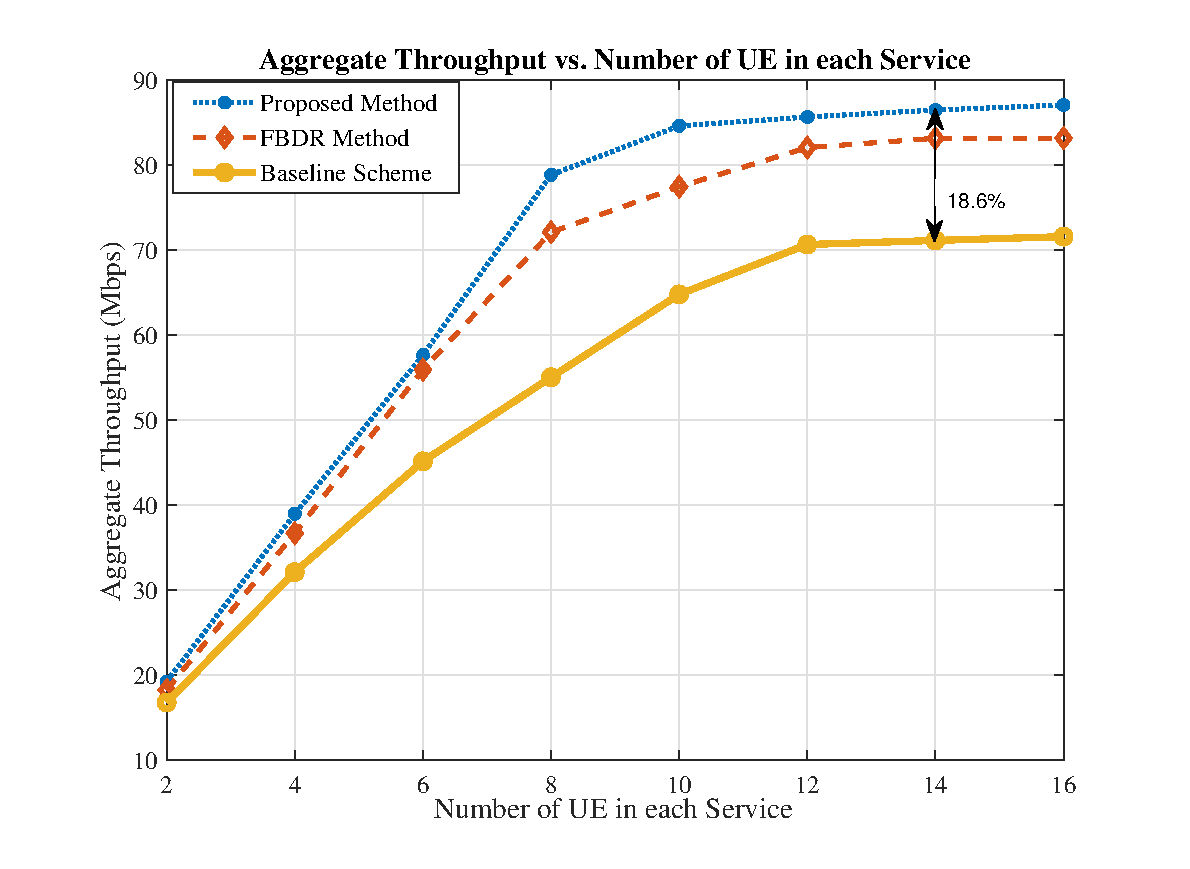
\includegraphics[scale = 0.4]{rate_ue1.eps}
    %\includegraphics[max height=30cm,max width=9.5cm]{Drawing15.eps}
    %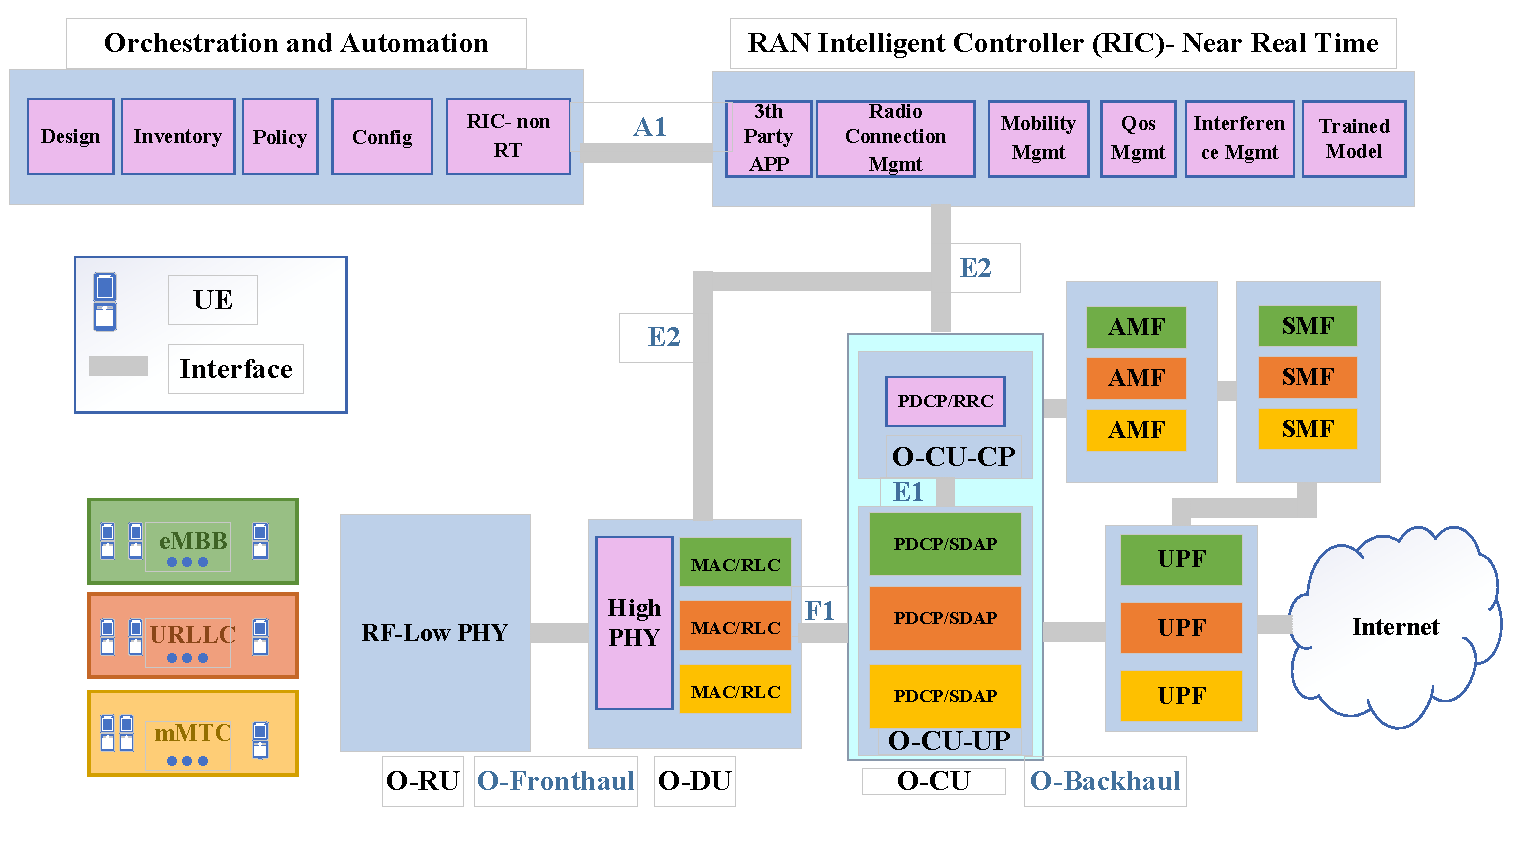
\includegraphics[width=\textwidth]{finalDraw.pdf}
  \caption{Aggregate Throughput vs. Number of UE in each Service }
  \label{fig:1}
\end{figure}

Assume we have two services of URLLC and mMTC. In figure \ref{fig:2} and \ref{fig:3}, the aggregate throughput (by considering the priority factor 
($\sum_s \sum_i \delta_s \bar{R}_{{u(s,i)}}$)) is depicted for two services URLLC and mMTC. Here we consider 4 UEs in each service. The other parameter is shown in table \ref{table:1a}.
The figure \ref{fig:2}, presented that by increasing the priority factor for URLLC, more resources is allocated to this service and the aggregate throughput of this service is increased and vice verse.
\begin{figure}
  \centering 
    \includegraphics[scale = 0.4]{mmtcurllc.eps}
    %\includegraphics[max height=30cm,max width=9.5cm]{Drawing15.eps}
    %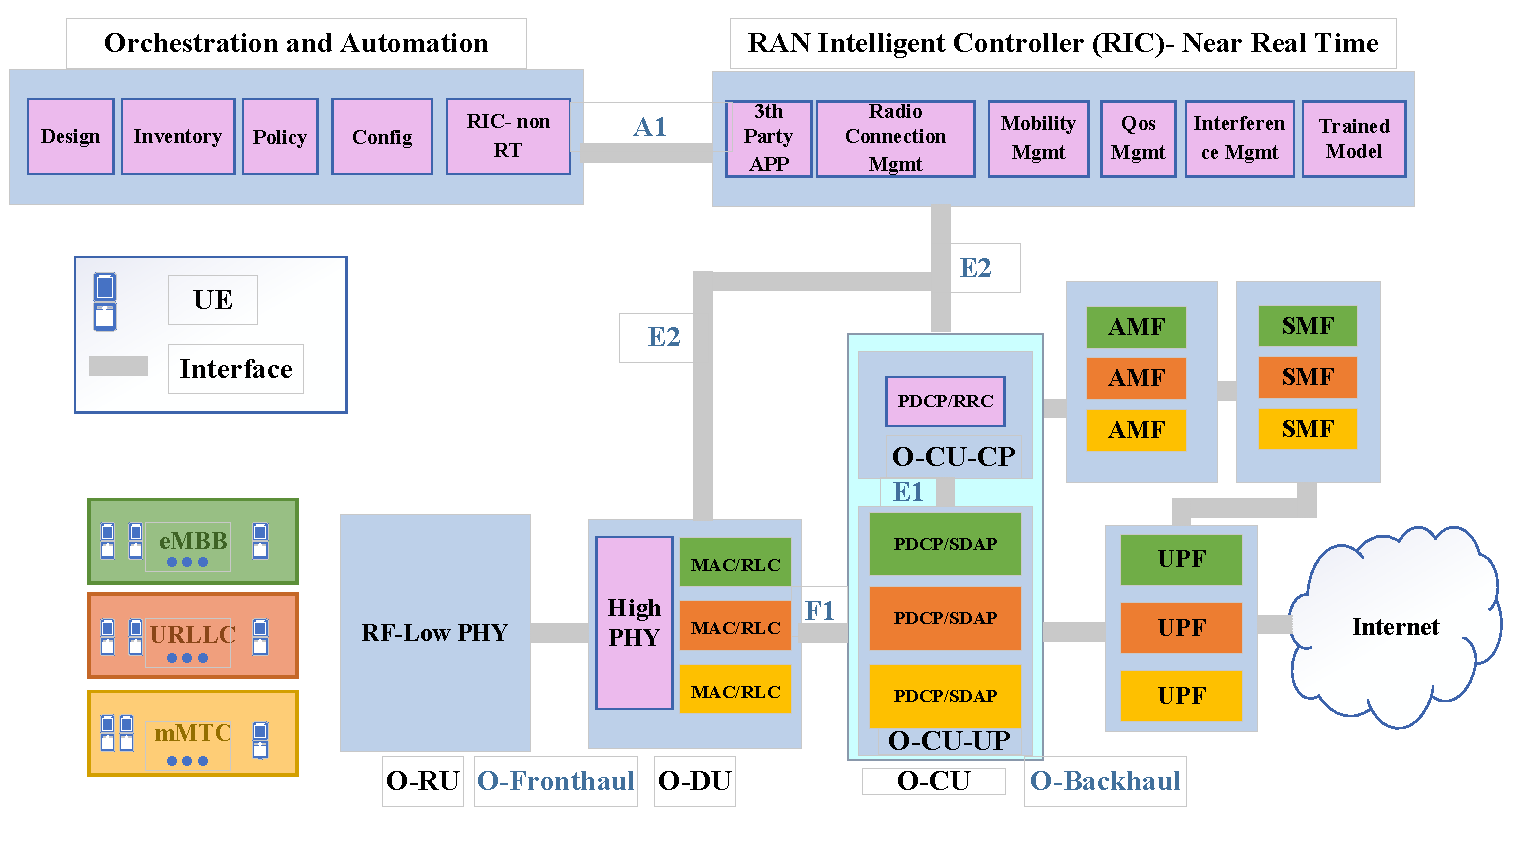
\includegraphics[width=\textwidth]{finalDraw.pdf}
  \caption{Aggregate Throughput for mMTC and URLLC vs. Priority of URLLC }
  \label{fig:2}
\end{figure}
In figure \ref{fig:3}, the total sum rate of URLLC and mMTC is shown vs. priority of URLLC. It is shown that the proposed method is much better than the baseline scheme. 
\begin{figure}
  \centering 
    \includegraphics[scale = 0.4]{sumRatePri.eps}
    %\includegraphics[max height=30cm,max width=9.5cm]{Drawing15.eps}
    %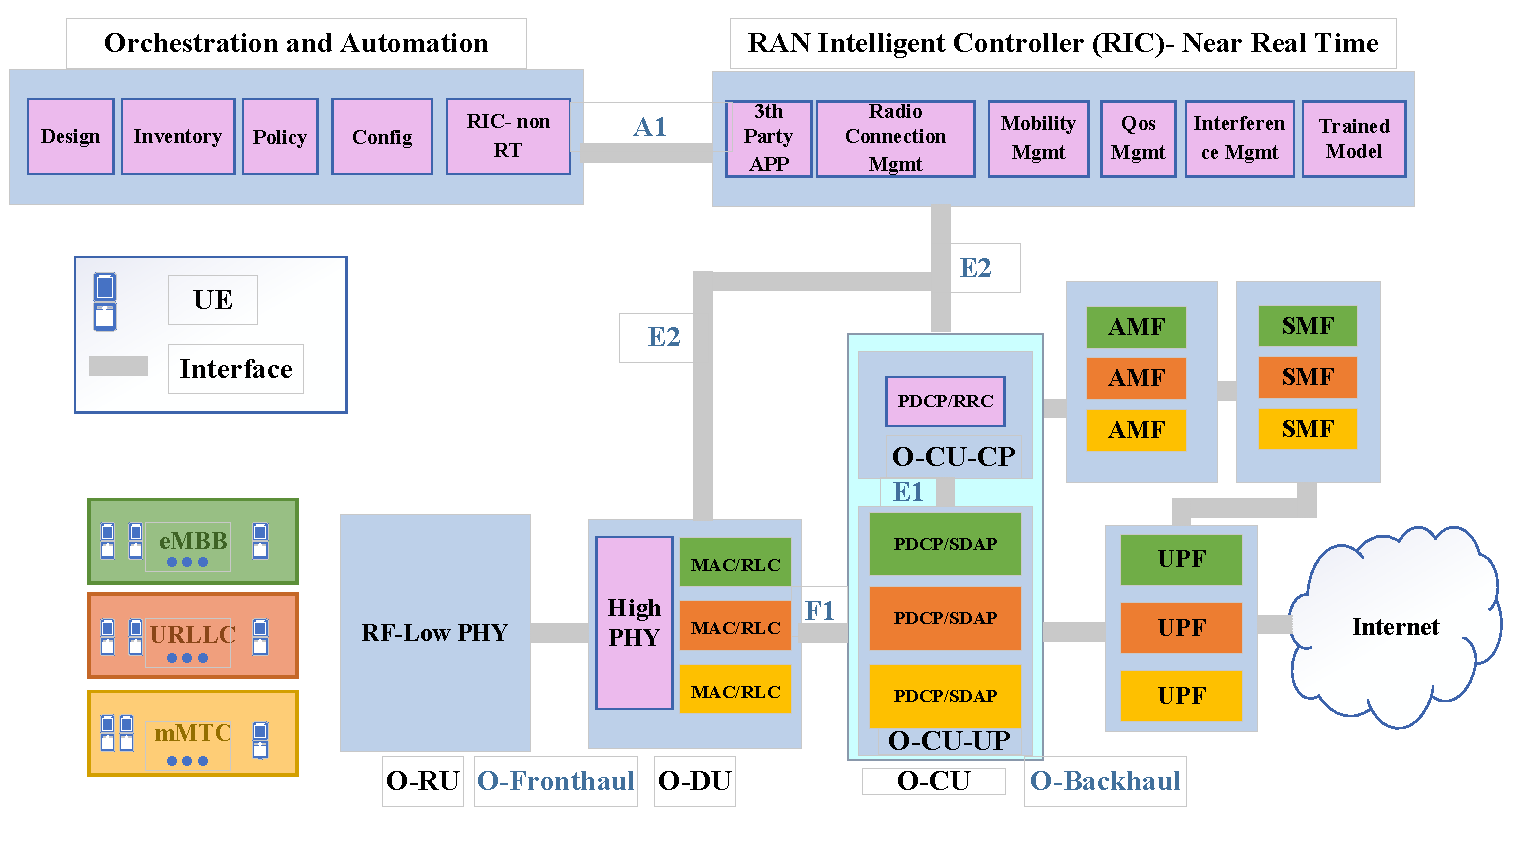
\includegraphics[width=\textwidth]{finalDraw.pdf}
  \caption{Aggregate Throughput of all services vs. Priority of URLLC}
  \label{fig:3}
\end{figure}
In figure \ref{fig:4}, the number of activated VNF for two different mean service time of a one eMBB service is depicted vs. mean arrival time. This figure, presented that as the mean arrival rate increases, the number of activated VNF increases. Moreover, the number of activated VNFs for the mean service rate of $\mu = 1.6Mbps$ is less than the number of activated VNFs for mean service rate of $\mu  =  0.8Mbps$.


\begin{figure}
  \centering 
    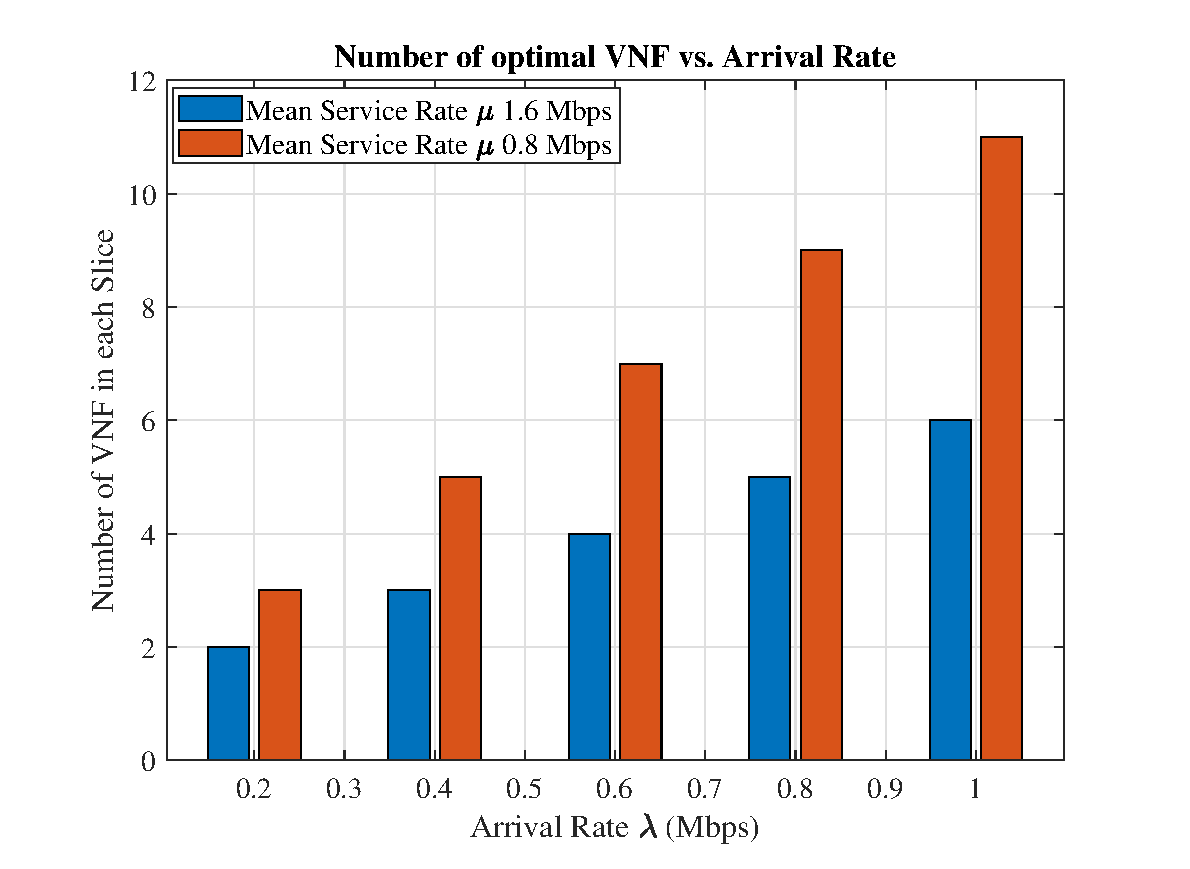
\includegraphics[scale = 0.4]{vnfNum.eps}
    %\includegraphics[max height=30cm,max width=9.5cm]{Drawing15.eps}
    %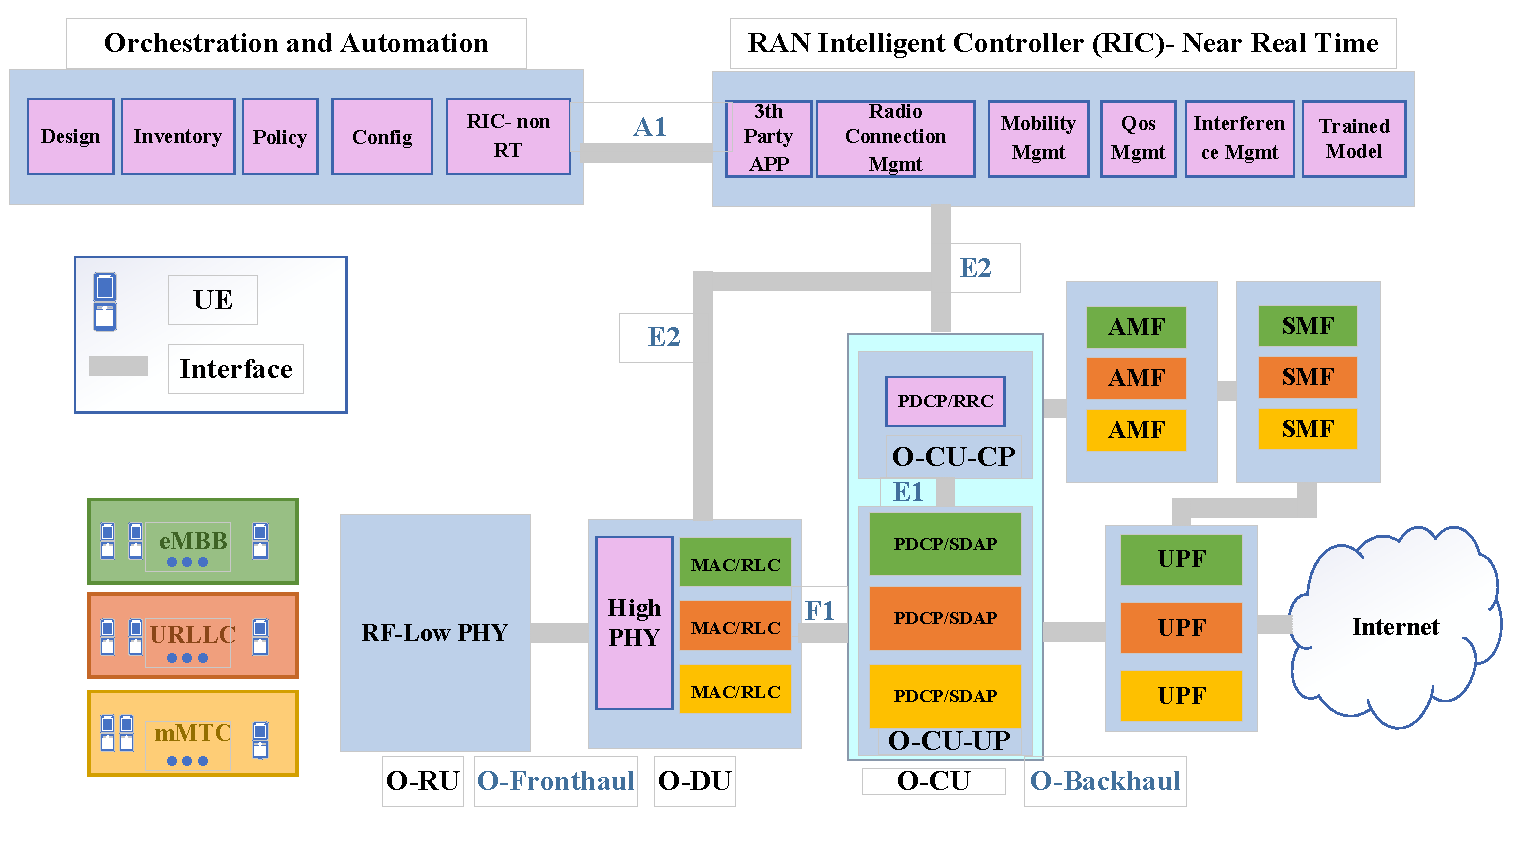
\includegraphics[width=\textwidth]{finalDraw.pdf}
  \caption{Number of activated VNF in each Service vs. Mean Arrival Rate(Mbps)}
  \label{fig:4}
\end{figure}




\section{Conclusion}\label{conc}
\bibliographystyle{IEEEtran}
\bibliography{ref}
\end{document} 